\documentclass[tikz,margin=10pt]{standalone}
\usetikzlibrary{arrows.meta,chains,decorations.pathreplacing}

\begin{document}

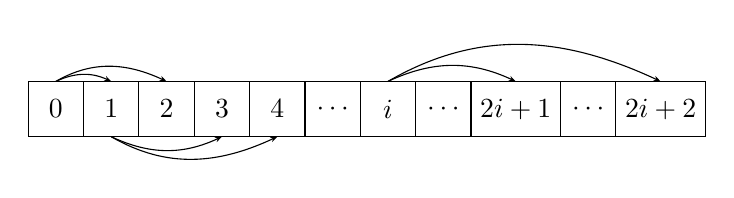
\begin{tikzpicture}[
        start chain = going right, node distance = 0pt, MyStyle/.style={draw, minimum width=2em, minimum height=2em, outer sep=0pt, on chain},
        ]
    \node [MyStyle] (0) {$0$};
    \node [MyStyle] (1) {$1$};
    \node [MyStyle] (2) {$2$};
    \node [MyStyle] (3) {$3$};
    \node [MyStyle] (4) {$4$};
    \node [MyStyle] (5) {$\cdots$};
    \node [MyStyle] (6) {$i$};
    \node [MyStyle] (7) {$\cdots$};
    \node [MyStyle] (8) {$2i+1$};
    \node [MyStyle] (9) {$\cdots$};
    \node [MyStyle] (10) {$2i+2$};
    \begin{scope}[-{Stealth[length = 2.5pt]}]
        \draw (0.north) [out=25, in=155] to (1.north);
        \draw (0.north) [out=30, in=155] to (2.north);
        \draw (1.south) [out=-25, in=-155] to (3.south);
        \draw (1.south) [out=-30, in=-155] to (4.south);
        \draw (6.north) [out=25, in=155] to (8.north);
        \draw (6.north) [out=30, in=155] to (10.north);

    \end{scope}
\end{tikzpicture}

\end{document}